\section{IT-Governance}

\subsection{Einordnung des Begriffes IT-Governance}
\label{section:einordung_it-governance}
IT-Governance ist der auf IT bezogene Teil der Corporate Governance. Somit ist IT-Governance ein Teil der Corporate Governance und Aufgabe der Unternehmensleitung und des gehobenen Managements. \footcite[Vgl.][445]{meyer_it-governance_2003}

Die Führung des Unternehmens ist durch Gesetze und Regulierungen zur Schaffung von Transparenz gezwungen. Diese Aufgaben werden u.a. unter dem Begriff Corporate Governance zusammengefasst. Dieser beschreibt die Unternehmensleitung und Unternehmensüberwachung, ausgerichtet an eine beständige Wertschöpfung. Compliance ist dabei die Übereinstimmung mit internen und externen Regeln wie z.B. Gesetzen. \footcite[Vgl.][356]{hofmann_it-governance_2010}
IT-Governance ist ein Teilgebiet der Corporate Governance, in welchem die IT bezogenen Aufgaben Anwendung finden. \footcite[Vgl.][10]{johannsen_it-governance_2006}

\subsection{Aufgaben des IT-Governance}

Die Kernaufgaben des IT-Governance sind das IT-Strategic-Alignment, also das Ausrichten der IT Strategie an der Strategie des Unternehmens, der Aspekt der Compliance durch z.B. rechtliche Regulierungen, der Messung von Erfolg/Performance, das Management von verfügbaren Resourcen und das Risikomanagement. Ebenso ist es sehr wichtig den wertschöpfenden Beitrag von IT zu erwähnen, welcher durch die IT-Governance sichergestellt werden soll. \footcite[Vgl.][14]{johannsen_it-governance_2006} Dadurch lässt sich die IT-Governance nicht von Coporate Governance trennen. Die strategische Ausrichtung der IT geht mit den Unternehmenszielen einher. Die Aufgaben des IT-Governance sind in \cref{fig:it-governance_aufgaben} auf der Seite \pageref{fig:it-governance_aufgaben} als Zyklus dargestellt. \footcite[Vgl.][446]{meyer_it-governance_2003} Beginnend mit der geschäftlichen Ausrichtung oder auch den Geschäftszielen werden Impulse für die Unternehmensstrategie geliefert und der daraus abgeleiteten IT-Strategie (IT-Strategic-Alignment). Aus dieser heraus soll das Unternehmen einen Mehrwert durch die IT erlangen. Zusammen mit dem Risikomanagement stellen diese Aufgaben die Implementierung der IT-Strategie dar. Der Zyklus endet mit der Erflogsmessung (IT-Performance). Diese kann wiederum neue Anreize für die Strategie liefern. Zentral steht das Ressourcenmanagement, welches eine wichtige Rolle in allen Aufgaben zu teil wird. \footcite[Vgl.][357\psq]{hofmann_it-governance_2010}

\begin{figure}[hbt]
\centering
\begin{minipage}[t]{1\textwidth} % Breite, z.B. 1\textwidth		
\caption{Aufgaben des IT-Governance} % Überschrift
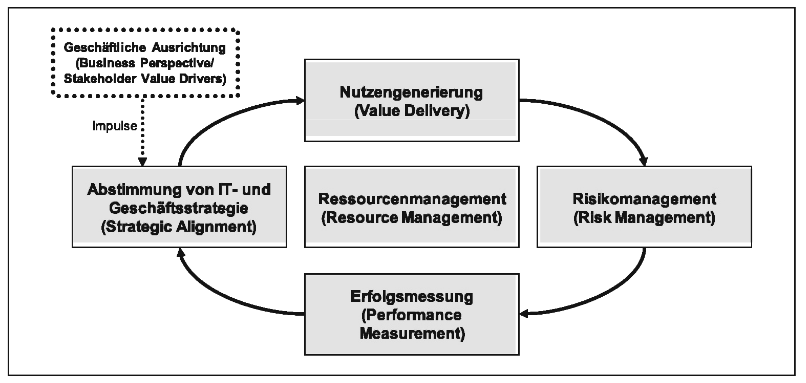
\includegraphics[width=1\textwidth]{img/Aufgabe_IT-Governance.png}\\
\source{\cite[357]{hofmann_it-governance_2010}} % Quelle
\label{fig:it-governance_aufgaben}
\end{minipage}
\end{figure}

Zum Beitrag der IT an dem Unternehmenserfolg muss diese auf die Strategie des Unternehmens angepasst werden, um Unternehmensziele zu erreichen. Dies ist unter dem Begriff IT-Strategic-Alignment zusammenzufassen. Somit muss die IT auf die geschäftlichen Aktivitäten ausgelegt und abgestimmt werden. \footcite[Vgl.][9]{johannsen_it-governance_2006}

Von der IT wird ein flexibler Beitrag zum Geschäftsergebnis erwartet. Dieser sollte direkt und messbar sein. Dabei wird IT in vielen Unternehmen noch als Cost-Center angesehen.\footcite[Vgl.][7]{johannsen_it-governance_2006}
  Dabei kann IT wertschöpfend und ermöglichend im Sinne von Prozessen und Geschäftszielen sein.\footcite[Vgl.][358]{hofmann_it-governance_2010}

Durch IT können Risiken wie z.B. Systemausfälle, unerlaubter Zugriff oder auch Budgetexplosionen entstehen. Die Aufgabe des Risikomanagements ist es, angemessen mit solchen Risiken umzugehen. Es existieren jedoch auch juristische Risiken durch Gesetze und Regulierungen. Deshalb ist das Risikomanagement eng mit dem Compliance bzw. IT-Complicance verzahnt. IT-Compliance sorgt für die Einhaltung von Regeln bezogen auf die IT. Regeln können externe Vorschriften vielseitiger Art sein aber auch Unternehmensinterne Regeln. \footcite[Vgl.][359\psq]{hofmann_it-governance_2010}

Der Wertbeitrag von IT muss gemessen werden, um zu bestimmen, ob die gesetzten Ziele erreicht wurden. Dies ist die Aufgabe der IT-Performance. Dabei kann die Messung des Einflusses der IT auf die Geschäftsziele auf Unternehmensebene durchaus schwierig sein. Das lokale messen der IT-Infrastruktur und IT-Systemen ist dahingegen durch definierte Maße gut bewertbar. \footcite[Vgl.][361]{hofmann_it-governance_2010}

Für die Entstehung, den Betrieb und die Wartung von IT werden Resourcen benötigt. Diese können z.B. Fachpersonal, Anwendungen, Infrastruktur oder Informationen sein. Der verantwortungsvolle Einsatz dieser Ressourcen ist ein wichtiger Erfolgsfaktor für die IT im Unternehmen. Somit ist ein Resourcemanagement eine unverzichtbare Aufgabe der IT-Governance.\footcite[Vgl.][362]{hofmann_it-governance_2010}

\subsection{Umsetzung von IT-Governance}

IT-Governance wird durch Strukturen und Prozesse angewendet. Zu erwähnen ist, dass interne und externe Faktoren dabei Konflikte verursachen können. Wichtig ist ebenfalls die Kommunikation zwischen der IT und dem Geschäft mit seinen geschäftliche Aktivitäten. Auf Grund der individualität von Unternehmen gibt es nicht die eine richtige Lösung. Jedes Unternehmen muss, die für sich richtigen Mechanismen, finden. \footcite[Vgl.][27]{de_haes_it_2004}
\nopagebreak
Für die Anwendung von IT-Governance können Frameworks genutzt werden. Diese beschreiben bereits Strukturen und Prozesse, welche für das Unternehmen genutzt werden kann. In der Literatur wird häufig das Framework \gls{COBIT} genannt. Diese Framework definiert bereits für eine Vielzahl von IT Prozessen und beschreibt welche Aktivitäten zu beachten sind. \gls{ITIL} ist ein weiteres Framework, welches auf die konkrete Implementierung von Aktivitäten abziehlt. 
Somit kann festgestellt werden, dass IT-Governance mithilfe von einem oder mehreren Frameworks implementiert werden kann und diese sich gegenseitig ergänzen können. \footcite[Vgl.][29\psqq]{de_haes_it_2004}

